%-------------------------------------------------------------------------------
\section{Motivation}\label{s:motivation}
%-------------------------------------------------------------------------------

This section reviews the potential benefits of serverless for
interactive workloads such as web applications, and presents
evidence that the {\problem} will need to be solved in order to
obtain those benefits.

\subsection{Web applications are a good fit for serverless}

Serverless is well suited to situations where load can vary rapidly
and is hard to predict, so that long-term cloud resource reservations
would lead to waste during low-load periods. Web applications often
fit this profile.

For example, consider a web site with 50,000 requests per day, each
request consuming 200 ms of CPU time and 128 MB of memory. The web
site is bursty in the sense that it has work only about a fifth of the
time. Running this web site on AWS Lambda would cost about \$1.60 per
month. The cheapest EC2 instance (which reserves compute resources)
costs just over \$3 per month. The expense-minimizing choice differs
depending on load level and degree of
burstyness~\cite{econ-of-serverless,trek10-blog},
but generally high load variation favors serverless.

Slowly-changing load can be handled by dynamic adjustment to long-term
reserved resources (e.g., EC2 instances), but such adjustments can take
multiple minutes~\cite{ec2-autoscaling} and are thus not suited to
rapid load variation.

\subsection{Serverless today}

\begin{figure}[t!]
  \centering
    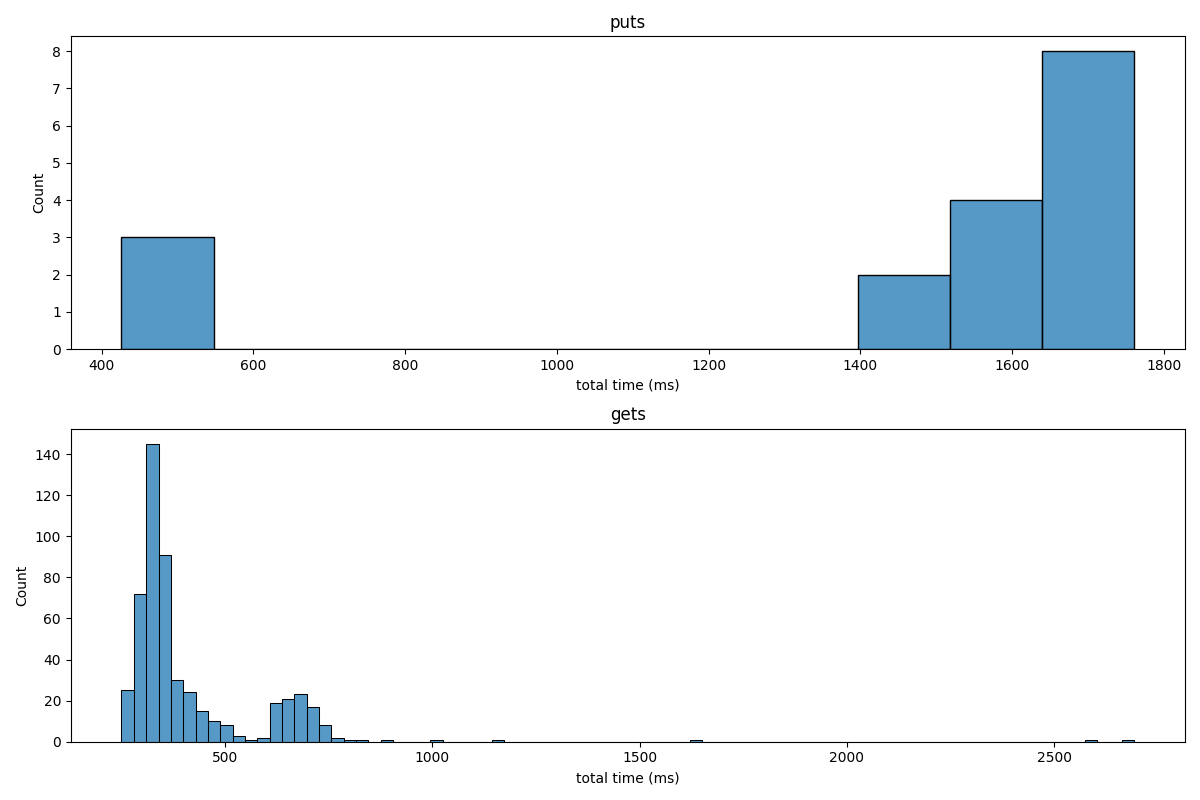
\includegraphics[width=8.5cm]{img/aws_webapp_times.png}
    \caption{Distribution of end-to-end durations for a simple function on AWS Lambda }
  \label{fig:lambda-total-durations}
\end{figure}


Serverless today does not provide the latencies that would be required of a web
server. We demonstrate this with a simple web application hosted on AWS that
uses the recommended serverless stack of: an ingress load balancer (API
Gateway), handler code (Lambda), and a database (DynamoDB). 

We model the distribution of gets/puts of real web applications, which have been
shown to have a skew of $\sim$95$\%$ gets, 5$\%$ puts. Gets fetch a table with
$~\sim$2K posts in it, and puts edit the content of one of those posts. We make
an API request every 30 seconds, and measure the end to end latencies of the
request within the AWS infrastructure using AWS XRay. The results are in
Figure~\ref{fig:lambda-total-durations}. The times for the puts are mostly long,
because puts are rare and so are usually hitting cold starts. The times for gets
have a wide distribution, though this cannot be caused by cold starts since
requests are usually 30 seconds apart. We can see from this distribution that
the observed end-to-end latencies are not acceptable for a web application. We
cannot, however, draw conclusions as to where this variation comes from.
\hmng{that's a little bit of a lie, we have a bit of a breakdown of these times.
Working on a graph for that rn, we can look at some candidates/discuss in the
meeting}

\hmng{how does this point relate to the crowding problem? Is it that we think
one of the reasons for the variance is the crowding problem? Would be great if
we could at least start to draw that connection, but will have lots of
conjecture. Ig this is what we did for the hotos draft, but feels like with the
other (more micro-benchmark-y) aws experiment is able to make a stronger
connection. Or is the point more separately proving that the state of the world
is such that it is implausible to run a web application on serverless? That's
kinda how I'm phrasing it here and how I read it }



\subsection{The \problem{}}

\begin{figure}[t!]
  \centering
    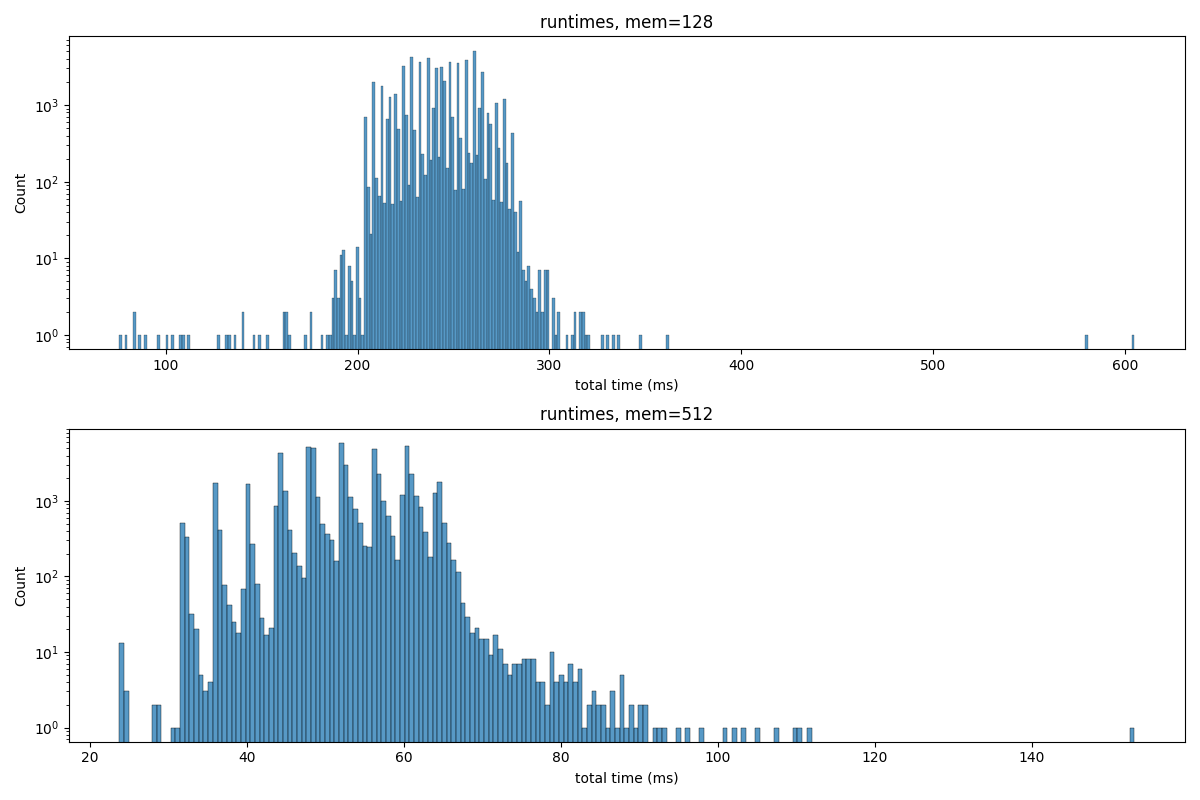
\includegraphics[width=8.5cm]{img/aws_cpubench_times.png}
    \caption{ Distribution of function wall-clock time passed during computation of a $\sim$20ms function on AWS lambda. The y axis is log scale. }
  \label{fig:lambda-cpu-bench}
\end{figure}

\begin{figure}[t!]
    \centering
      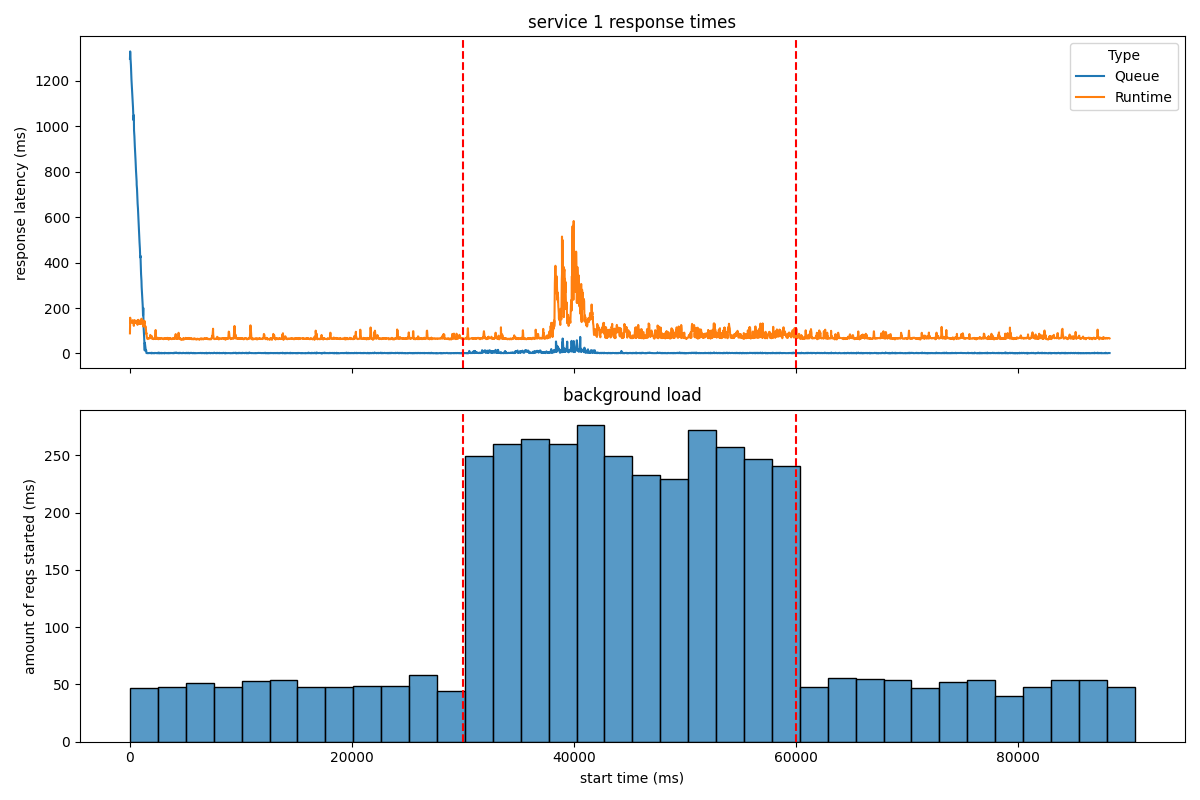
\includegraphics[width=8.5cm]{img/knative_loadexp_times.png}
      \caption{Distribution of end-to-end durations broken down by
        queuing (blue) and runtime (orange) delay for a simple function on
        knative.}
    \label{fig:knative}
\end{figure}

Cloud providers like AWS are motivated to keep their compute hardware as busy as
possible, in order to avoid waste and reduce costs. In a non-reservation system
like serverless, if the average load is near capacity (to minimize average
waste), the peak load will be above capacity, imposing either queuing or
time-sharing delays on functions. The \problem{} is that this undesirable
behavior of queueing/delay happens indiscriminately in current serverless
systems, meaning that a function's latency is affected by the load of other
potentially less latency sensitive functions, and even other tenants' functions.

Measurements of a cpu-bound serverless function in AWS Lambda show evidence of
this \problem{}. The function we run mainly consists of a double for loop that
computes a matrix multiplication. It measures the wall clock time that passes
between the beginning and the end of the loop, as well as the cpu time that it
got. In AWS, the fractional amount of CPU time a function gets is tied to the
maximum amount of memory it configures, so we run the function in two settings:
once with memory a limit of 128 MB, and once with 512 MB. We invoke each
function every 30 seconds for 24 hours.

The results are in Figure~\ref{fig:lambda-cpu-bench}; not pictured are the
cpu-times of each run, which hold steady at $\sim$ 20ms. At a glance, the
\problem{} is evident: the wall-clock time it takes to run the exact same code
varies significantly. The absolute size of the spread for the 512MB
configuration is about half the size of the 128MB configuration's.
\hmng{actually, this makes me curious what happens if we go up to 1 vCPU. Could
there be a graph relating spread size to mem config/vCPU amt?} A separate
interesting artifact in the graph are the spikes, prominent even in a log-scale
y axis depiction. The spikes occur every 4ms, which is the default linux
scheduling interval. The likely conclusion is that each spike represents a
number of scheduling cycles passed before the function was able to finish, with
times in between being caused by an intermediate function not using its whole
4ms scheduling interval.


We find that the crowding problem also happens in open-source serverless
systems. One such system is Knative,\cite{knative}, which runs a Kubernetes pod
for each function; pods time-share the provider's servers. Knative assigns
function invocations to pods until the pods are fully loaded, and then queues
invocations until a pod has capacity or the autoscaler has created new pod. We
run an experiment with Knative in which we generate a steady stream of
background functions and periodically invoke a latency-sensitive function that
computes for $\sim$50ms. Figure~\ref{fig:knative} shows how the end-to-end
request durations for the foreground function change in the face of a spike in
load of the background traffic. The graph breaks down the duration into queuing
and runtime (i.e., the time from the first to last line of code of the
function). It shows that both become more variable when the background traffic
load is higher, with spikes in queueing time and variable as well as overall
significantly higher runtimes. \hmng{ queueing immediately becomes a little more
variable, but only really starts spiking a little less than one second later
which is also when runtimes spike (what is happening there?). Half a second
later runtimes go back down again, though stay more variable, and queueing
stabilizes (presumably this is that the new pods have been started?). Do we want
a more aggressive experiment where background load becomes so high that capcity
is overall exceeded, so that even when new pods are started the times stay
higher? Becuase this is kind of making the point more about auto scaling being
slow, which is also crowding but while its waiting for stuff to start}

The takeaway here is that the duration of latency sensitive functions is
affected significantly by the background load, which leads to both queueing and
time-sharing delay: the \problem{}.
